% Needed for strikethrough with \st
\usepackage{soul}

\usepackage{tikz}
\usetikzlibrary{arrows.meta,positioning}

\title{ITC8280 Fundamentals of Cryptography}
\subtitle{Introduction to cryptography}
\date{\today}
\author{Taaniel Kraavi}
\institute%
{%
  \textit{School of Information Technologies}\\
  \textit{Tallinn University of Technology}
}

\begin{document}
\begin{frame}
  \titlepage
\end{frame}

\begin{frame}{What's in a name?}
  \begin{itemize}[<+(1)->]
    \item Historically: the art of codes
    \item Cornerstone of computer and information security
    \item Secures communications in presence of adversarial behaviour
    \item Replaces a hard problem with a another problem
    \par
    \begin{itemize}
      \item Key-management and/or mathematics
    \end{itemize}
    \item Cryptography $\neq$ cryptocurrency / blockchain
  \end{itemize}
\end{frame}

\begin{frame}{CIA and cryptography}
  \pause
  \begin{itemize}
    \item Confidentiality
    \item Integrity
    \item \st{Availability}
    \pause
    \item Authenticity
    \item Non-repudiation
  \end{itemize}

  \vspace{1em}

  \pause
  Availability is typically assumed: a communication channel exists
  \begin{itemize}[<+(1)->]
    \item Cryptography is about securing communication, not hiding it
    \item Steganography: covert communication, hiding data within a medium
  \end{itemize}
\end{frame}

\begin{frame}{Extended CIA triad}
  \begin{itemize}
    \pause
    \item Confidentiality
    \begin{itemize}
      \item Secrecy of content
    \end{itemize}
    \pause
    \item Integrity
    \begin{itemize}
      \item Correctness of content
      \item Change detection, not prevention
    \end{itemize}
    \pause
    \item Authenticity
    \begin{itemize}
      \item Correctness of claimed content origin
      \begin{itemize}
        \item Link to a key, not necessarily an identity
      \end{itemize}
      \item Implies integrity: change of message $=$ change of origin
    \end{itemize}
    \pause
    \item Non-repudiation
    \begin{itemize}
      \item Accountability: sender cannot (plausibly) deny their action
      \item Public verifiability (typically)
    \end{itemize}
  \end{itemize}
\end{frame}

\begin{frame}{Ladder of abstraction}

  \pause
  \begin{itemize}
    \item \textbf{Many levels of building blocks}
    \pause
    \begin{itemize}
      \item Mathematical foundations
      \item Cryptographic primitives
      \item Cryptographic protocols
    \end{itemize}

    \vspace*{1em}

    \pause
    \item \textbf{Implementation details complicate security reasoning}
    \pause
    \begin{itemize}
      \item Abstractions highlight desirable properties.
      \item Some of these properties are security-relevant.
      \item Security is defined via these properties in an adversary model.
      \par
      \begin{itemize}
        \item What are the adversary's capabilities and goals?
      \end{itemize}
    \end{itemize}
  \end{itemize}

  \vspace*{1em}

  \pause
  Implementation security must be addressed separately.
\end{frame}

\begin{frame}{Defining security}
  \textbf{Two approaches to security}
  \begin{itemize}
    \pause
    \item Heuristic security / best-effort design
    \begin{itemize}
      \item Resistance to known attacks, test of time, security \enquote{margins}
    \end{itemize}
    \pause
    \item Provable security
    \begin{itemize}
      \pause
      \item Proofs that rely on problems believed to be hard
      \begin{itemize}
        \item Computational hardness assumptions about mathematical problems
        \item Security reductions: if problem $P$ is hard then protocol $\Pi$ is secure
      \end{itemize}

      \pause
      \item Information-theoretic security proofs
      \begin{itemize}
        \item Proof of unconditional security
        \item No hardness assumptions needed
      \end{itemize}
    \end{itemize}

    \vspace*{1em}

    \pause
    NB! Careful with nomenclature: the term \enquote{provable} can be confusing
  \end{itemize}
\end{frame}

\begin{frame}{Defining security}
  \textbf{Two types of security}
  \begin{itemize}[<+(1)->]
    \item Conditional --- computational
    \begin{itemize}
      \item Secure against bounded adversaries
    \end{itemize}
    \item Unconditional\textsuperscript{*} --- information-theoretic
    \begin{itemize}
      \item Secure against unbounded adversaries
      \item Caveat: it is conditional in the larger context
      \par
      \begin{itemize}
        \item A \emph{trust model} must be specified
        \item Proper procedure must be followed
      \end{itemize}
    \end{itemize}
  \end{itemize}
\end{frame}

\begin{frame}{Intractability}
  \begin{itemize}
    \item \textbf{Practical security is based on \emph{intractability}.}
    \begin{itemize}[<+(1)->]
      \item It is \emph{infeasible} to solve a problem in practice.
      \item We are \emph{computationally bounded}: limited by time and space.
    \end{itemize}

    \vspace*{1em}

    \pause
    \item The feasibility bound evolves:
    \begin{itemize}[<+(1)->]
      \item Humans keep pushing the boundary of what is feasible.
      \item Dedicated tooling significantly improves attack feasibility (e.g. ASICs).
    \end{itemize}
    
    \vspace*{1em}

    \pause
    \item Never assume that parameters are secure: verify with experts.
    \begin{itemize}[<+(1)->]
      \item Recommendations by ANSSI, BSI, NIST\textsuperscript{*}.
      \item Independent opinions of respected cryptographers.
      \item Err on the side of caution.
      \item What is safe today may not be safe soon.
    \end{itemize}
  \end{itemize}
\end{frame}

\begin{frame}
  \frametitle{Kerckhoff's principle}

  \pause
  \textbf{Definition.}
  A cryptographic system should be secure even if everything about the system, except the key, is public knowledge.

  \vspace*{1em}

  \pause
  \textbf{Interpretation.}
  A system's security should depend on the secrecy of its usage parameters, not of its algorithms.
\end{frame}

\begin{frame}
  \frametitle{Cryptosystems}
  \framesubtitle{Informal introduction}

  \pause
  Let $m$ be some message called the \emph{plaintext}.

  \vspace*{1em}

  \pause
  A cryptosystem is a triple of algorithms $(\GEN,\ENC,\DEC)$ where
  \begin{itemize}[<+(1)->]
    \item $\GEN$ is a key generation algorithm
    \item $\ENC$ is an encryption algorithm: $c\gets\ENC_{\textit{key}}(m)$
    \item $\DEC$ is a decryption algorithm: $m\gets\DEC_{\textit{key}}(c)$
  \end{itemize}

  \vspace*{1em}

  \pause
  The output of the encryption $c\gets\ENC_{\textit{key}}(m)$ is called the \emph{ciphertext}.

  \vspace*{1em}

  \pause
  The cryptosystem is functional if $\DEC_{\textit{key}}(\ENC_{\textit{key}}(m))=m$.
\end{frame}

\begin{frame}[c]
  \centering
  What makes a cryptosystem secure?
\end{frame}

\begin{frame}
  \frametitle{Attack models}

  \begin{itemize}[<+(1)->]
    \item Ciphertext-only attack
    \begin{itemize}
      \item You only know a ciphertext.
    \end{itemize}
    \item Known-plaintext attack (KPA)
    \begin{itemize}
      \item You are given a ciphertext--plaintext pair.
    \end{itemize}
    \item Chosen-plaintext attack (CPA)
    \begin{itemize}
      \item You are given ciphertexts for plaintexts you provide.
    \end{itemize}
    \item Chosen-ciphertext attack (CCA)
    \begin{itemize}
      \item You are given plaintexts for ciphertexts you provide.
    \end{itemize}
  \end{itemize}
\end{frame}

\begin{frame}{Strength of attack models}
  \begin{figure}
  \centering
  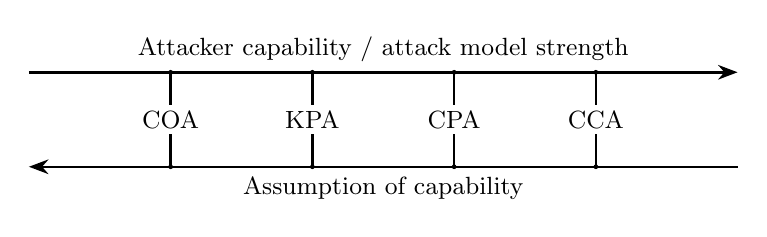
\begin{tikzpicture}[>=Stealth, line width=0.9pt]
    \coordinate (L) at (0,0);
    \coordinate (R) at (9,0);

    \def\TopY{0.6}    % y of top line
    \def\BotY{-0.6}   % y of bottom line

    \def\BarTop{0.6}
    \def\BarBot{-0.6}

    \def\DX{1.8} % = 9/5
    \coordinate (B1) at (0 + 1*\DX, 0);
    \coordinate (B2) at (0 + 2*\DX, 0);
    \coordinate (B3) at (0 + 3*\DX, 0);
    \coordinate (B4) at (0 + 4*\DX, 0);

    \draw[->] (0,\TopY) -- (9,\TopY) node[midway, above, font=\small]{Attacker capability / attack model strength};
    \draw[->] (9,\BotY) -- (0,\BotY) node[midway, below, font=\small]{Assumption of capability};

    \foreach \X in {1,2,3,4} {
      \pgfmathsetmacro{\xx}{\X*\DX}
      \draw (\xx,\BarBot) -- (\xx,\BarTop);
      \fill (\xx,\BarTop) circle (0.03);
      \fill (\xx,\BarBot) circle (0.03);
    }

    \node[font=\small, fill=white, inner sep=2pt] at (4*\DX, 0) {CCA};
    \node[font=\small, fill=white, inner sep=2pt] at (3*\DX, 0) {CPA};
    \node[font=\small, fill=white, inner sep=2pt] at (2*\DX, 0) {KPA};
    \node[font=\small, fill=white, inner sep=2pt] at (1*\DX, 0) {COA};
  \end{tikzpicture}
  \end{figure}

  \pause
  Stronger attack models encompass weaker ones, thus
  \begin{itemize}[<+(1)->]
    \item Successful attack under a weaker model $\implies$ success under a stronger model
    \begin{itemize}
      \item E.g. a scheme broken under CPA is also broken under CCA
    \end{itemize}
    \item Security against a stronger model $\implies$ security against all weaker models
    \begin{itemize}
      \item E.g. a scheme safe under CCA is safe under CPA
    \end{itemize}
  \end{itemize}
\end{frame}

\begin{frame}{Strength of assumptions}
  \begin{figure}
  \centering
  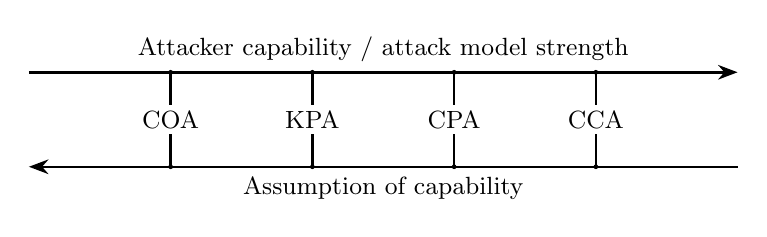
\begin{tikzpicture}[>=Stealth, line width=0.9pt]
    \coordinate (L) at (0,0);
    \coordinate (R) at (9,0);

    \def\TopY{0.6}    % y of top line
    \def\BotY{-0.6}   % y of bottom line

    \def\BarTop{0.6}
    \def\BarBot{-0.6}

    \def\DX{1.8} % = 9/5
    \coordinate (B1) at (0 + 1*\DX, 0);
    \coordinate (B2) at (0 + 2*\DX, 0);
    \coordinate (B3) at (0 + 3*\DX, 0);
    \coordinate (B4) at (0 + 4*\DX, 0);

    \draw[->] (0,\TopY) -- (9,\TopY) node[midway, above, font=\small]{Attacker capability / attack model strength};
    \draw[->] (9,\BotY) -- (0,\BotY) node[midway, below, font=\small]{Assumption of capability};

    \foreach \X in {1,2,3,4} {
      \pgfmathsetmacro{\xx}{\X*\DX}
      \draw (\xx,\BarBot) -- (\xx,\BarTop);
      \fill (\xx,\BarTop) circle (0.03);
      \fill (\xx,\BarBot) circle (0.03);
    }

    \node[font=\small, fill=white, inner sep=2pt] at (4*\DX, 0) {CCA};
    \node[font=\small, fill=white, inner sep=2pt] at (3*\DX, 0) {CPA};
    \node[font=\small, fill=white, inner sep=2pt] at (2*\DX, 0) {KPA};
    \node[font=\small, fill=white, inner sep=2pt] at (1*\DX, 0) {COA};
  \end{tikzpicture}
  \end{figure}

  Adversaries may be highly capable:
  \begin{itemize}[<+(1)->]
    \item Weaker attack model $\implies$ more adversarial restrictions
    \item More restrictions $\implies$ stronger assumption (about fewer capabilities)
    \item Stronger assumption $\implies$ weaker security claim
    \par
    \begin{itemize}
      \item Adversary more powerful than assumed: security may no longer hold
    \end{itemize}
  \end{itemize}
\end{frame}

\begin{frame}{Simple ciphers}
  Well-known examples include:
  \pause
  \begin{itemize}
    \item Substitution ciphers (monoalphabetic)
    \begin{itemize}
      \item shift cipher, simple substitution cipher
    \end{itemize}
    \pause
    \item Substitution ciphers (polyalphabetic)
    \begin{itemize}
      \item Vigenère cipher
    \end{itemize}
    \pause
    \item Transposition ciphers
    \begin{itemize}
      \item simple permutation cipher, scytale
    \end{itemize}
  \end{itemize}

  \vspace{1em}

  \pause
  More generally:
  \begin{itemize}
    \item In a substitution cipher values change.
    \item In a transposition cipher positions change.
  \end{itemize}

\end{frame}

\begin{frame}{Shannon's design principles}
  \begin{itemize}
    \pause
    \item \textbf{Confusion}
    \begin{itemize}
      \item Obfuscates the relation between ciphertext \& key.
      \item Makes key extraction difficult.
      \pause
      \item Provided by substitution, e.g. S-boxes.
    \end{itemize}

    \vspace*{1em}

    \pause
    \item \textbf{Diffusion}
    \begin{itemize}
      \item Obfuscates the statistical relation between plaintext \& ciphertext.
      \item Makes statistical attacks difficult.
      \pause
      \item Provided by permutation, e.g. P-boxes.
    \end{itemize}

    \vspace*{2em}

    \pause
    Useful, but neither sufficient nor strictly necessary for security.
    \begin{itemize}[<+(1)->]
      \item Used in the design of block ciphers, e.g. SP-networks (SPN).
    \end{itemize}
  \end{itemize}
\end{frame}

\end{document}
